\chapter{Escolha do jogo}

Para a escolha do jogo foi pensado em suprir a falta de jogos de corrida no mercado brasileiro, visto que o Brasil não possui muitos jogos de corrida, e os que existem são de empresas estrangeiras. Além disso, outros alunos do curso de Ciência da Computação da USP já haviam desenvolvido jogos em OpenGL onde foi possível, com o passar do tempo, aprimorar o conhecimento e a experiência com a biblioteca.

Com o uso do OpenGL e a utilização de memória gráfica, foi possível desenvolver um jogo de corrida em 3D, rápido e dinâmico, com a possibilidade de adicionar novos elementos e funcionalidades ao jogo.

\section{Gênero do jogo}

Além de tudo isso, por uma questão de preferência pessoal, foi escolhido um estilo de jogo que é muito popular e de grande apreço pelo autor, o estilo de corrida de Kart.

Vários jogos de corrida de Kart já foram desenvolvidos, como \textit{Mario Kart}, \textit{Crash Team Racing}, \textit{Blur}, \textit{Rock \& Roll Racing} entre vários outros. Todos esses jogos possuem características únicas e são muito divertidos de jogar, o que torna o gênero de corrida de Kart, entendido aqui como jogos de corrida com combate e trapaça, muito popular e apreciado por muitos jogadores.

\subsection{Mario Kart}

\textit{Mario Kart} é uma série de jogos de corrida de Kart desenvolvida e publicada pela Nintendo. O primeiro jogo da série foi lançado em 1992 para o Super Nintendo Entertainment System (SNES) e desde então a série se tornou uma das mais populares e bem-sucedidas da Nintendo.

Os jogos da série \textit{Mario Kart} são conhecidos por sua jogabilidade acessível e dinâmica, que combina elementos de corrida e combate, e por seus personagens carismáticos e coloridos, como Mario, Luigi, Peach, Bowser, Donkey Kong, Yoshi, entre outros.

\begin{figure}[H]
    \centering
    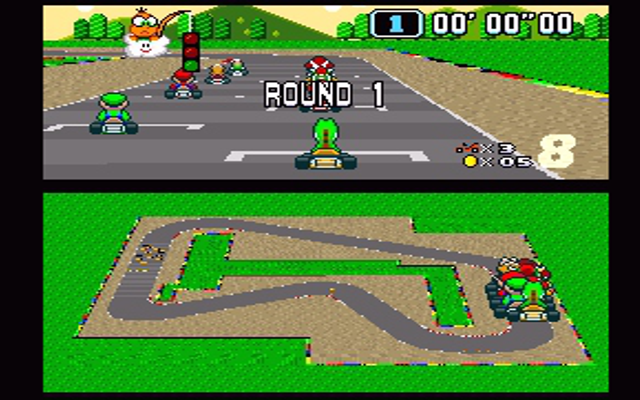
\includegraphics[width=0.8\textwidth]{figuras/Mario Kart.png}
    \caption{Mario Kart. \cite{marioKart}}
    \label{fig:mario-kart}
\end{figure}

\subsection{Crash Team Racing}

\textit{Crash Team Racing} é um jogo de corrida de Kart desenvolvido pela Naughty Dog e publicado pela Sony Computer Entertainment para o PlayStation em 1999. O jogo é conhecido por sua jogabilidade desafiadora e por seus personagens carismáticos, como Crash Bandicoot, Dr. Neo Cortex, Coco Bandicoot, entre outros.

\begin{figure}[H]
    \centering
    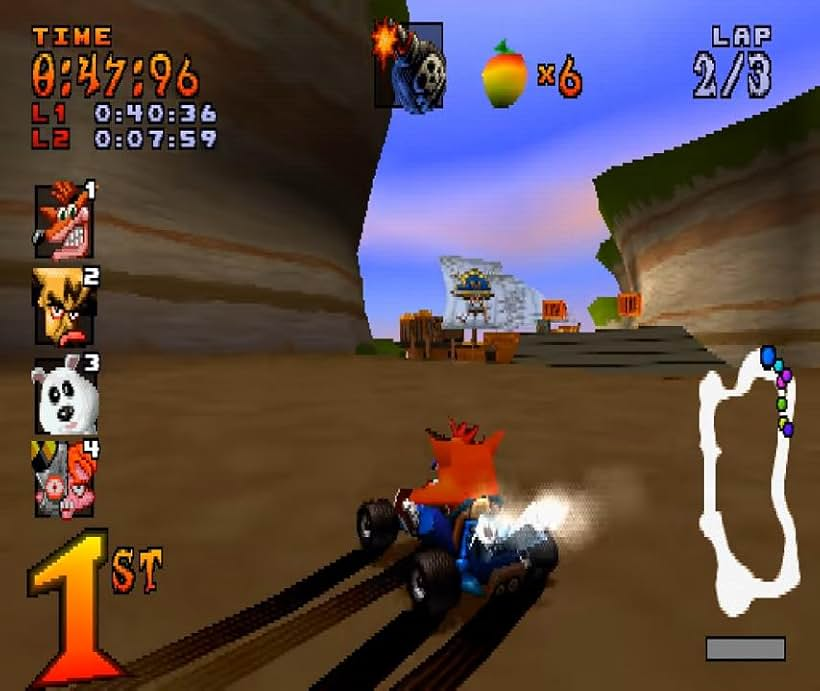
\includegraphics[width=0.8\textwidth]{figuras/Crash Team Racing.jpg}
    \caption{Crash Team Racing. \cite{crashTeamRacing}}
    \label{fig:crash-team-racing}
\end{figure}

Um de seus principais diferenciais é o modo de jogo \textit{Adventure}, onde o jogador deve competir em várias pistas e desafios para coletar cristais e chaves e derrotar Nitros Oxide, o vilão do jogo.

\textit{Crash Team Racing} foi um grande sucesso de crítica e público e se tornou um dos jogos de corrida de Kart mais populares do PlayStation, com milhões de cópias vendidas em todo o mundo.

Em 2019, a Activision lançou um remake do jogo, chamado \textit{Crash Team Racing Nitro-Fueled}, para PlayStation 4, Xbox One, Nintendo Switch e PC, que foi muito bem recebido pela crítica e pelos fãs da série, o que mostra o quanto o estilo de jogo é relevante e popular até hoje.

\begin{figure}[H]
    \centering
    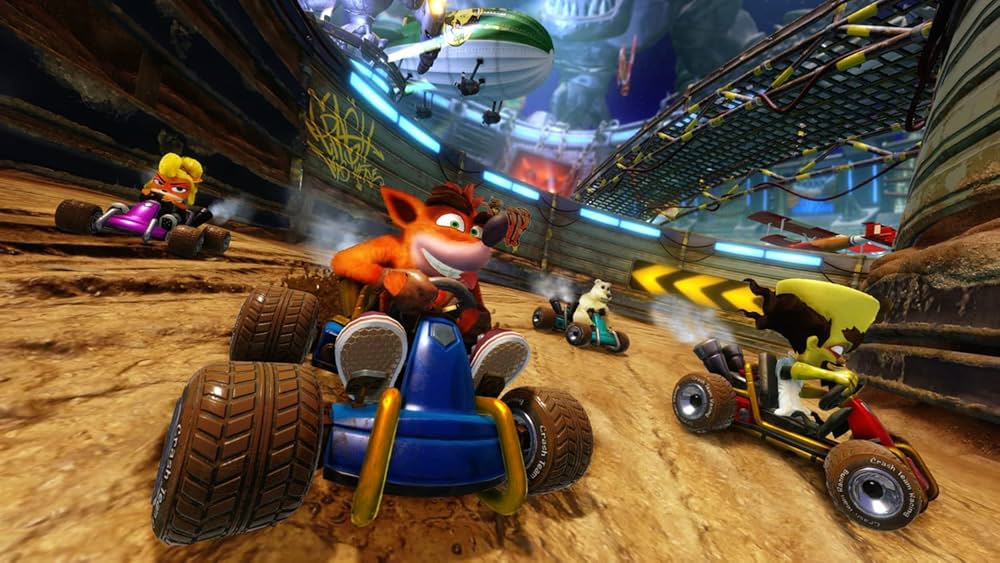
\includegraphics[width=0.8\textwidth]{figuras/Crash Team Racing Nitro Fueled.jpg}
    \caption{Crash Team Racing Nitro-Fueled. \cite{crashTeamRacingNitroFueled}}
    \label{fig:crash-team-racing-nitro-fueled}
\end{figure}

\subsection{Blur}

\textit{Blur} é um jogo de corrida de Kart desenvolvido pela Bizarre Creations e publicado pela Activision para PlayStation 3, Xbox 360 e PC em 2010. O jogo é conhecido por sua jogabilidade arcade e por seus gráficos realistas, que combinam elementos de corrida e combate.

Seu principal diferencial é o seu combate veicular, onde os jogadores podem usar power-ups para atacar e defender seus oponentes, como mísseis, minas, escudos, entre outros.

Nesse estilo de jogo, o jogador pode escolher entre vários carros e pilotos, cada um com suas próprias habilidades e características únicas, e competir em várias pistas e modos de jogo, como o modo carreira, modo de múltiplos jogadores, entre outros.

Ele não é tão semelhante aos jogos de corrida de Kart tradicionais, mas é um jogo muito divertido e desafiador, que combina elementos de corrida e combate de uma forma única e inovadora, com um tema mais adulto e realista.

\begin{figure}[H]
    \centering
    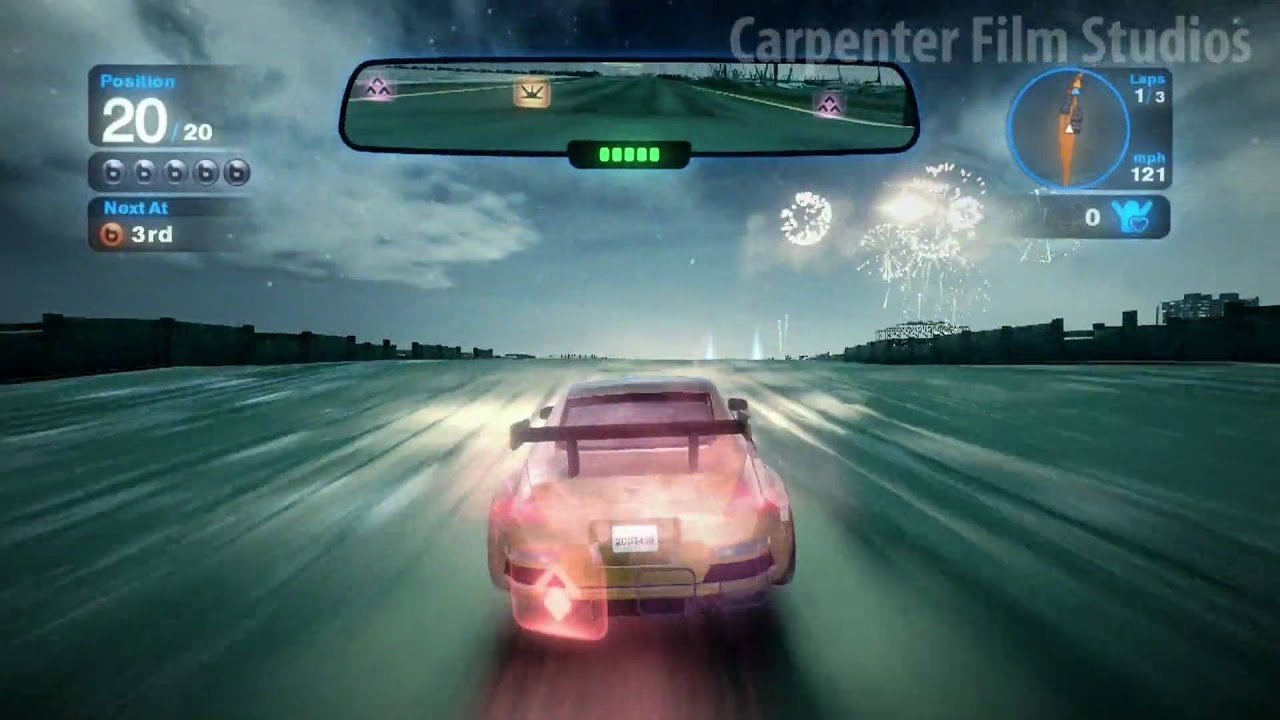
\includegraphics[width=0.8\textwidth]{figuras/Blur.jpg}
    \caption{Blur. \cite{blur}}
    \label{fig:blur}
\end{figure}

\subsection{Rock \& Roll Racing}

\textit{Rock \& Roll Racing} é um jogo de corrida de Kart desenvolvido pela Silicon \& Synapse (atual Blizzard Entertainment) e publicado pela Interplay Productions para o Super Nintendo Entertainment System (SNES) e Mega Drive em 1993.

O jogo é conhecido por sua jogabilidade acessível e dinâmica, que combina elementos de corrida e combate, e por sua trilha sonora de \textit{rock and roll}, que inclui músicas de bandas como Black Sabbath, Deep Purple, Steppenwolf, entre outras.

A ideia do jogo é envolver o jogador numa corrida de Kart futurista, onde ele deve competir em várias pistas e desafios para ganhar dinheiro e comprar novos carros e armas, que podem ser usados para atacar e defender seus oponentes.

Diferente dos outros jogos de corrida de Kart, \textit{Rock \& Roll Racing} é um jogo de corrida de Kart isométrico, onde o jogador vê o carro de cima, o que dá uma perspectiva diferente e única ao jogo.

\begin{figure}[H]
    \centering
    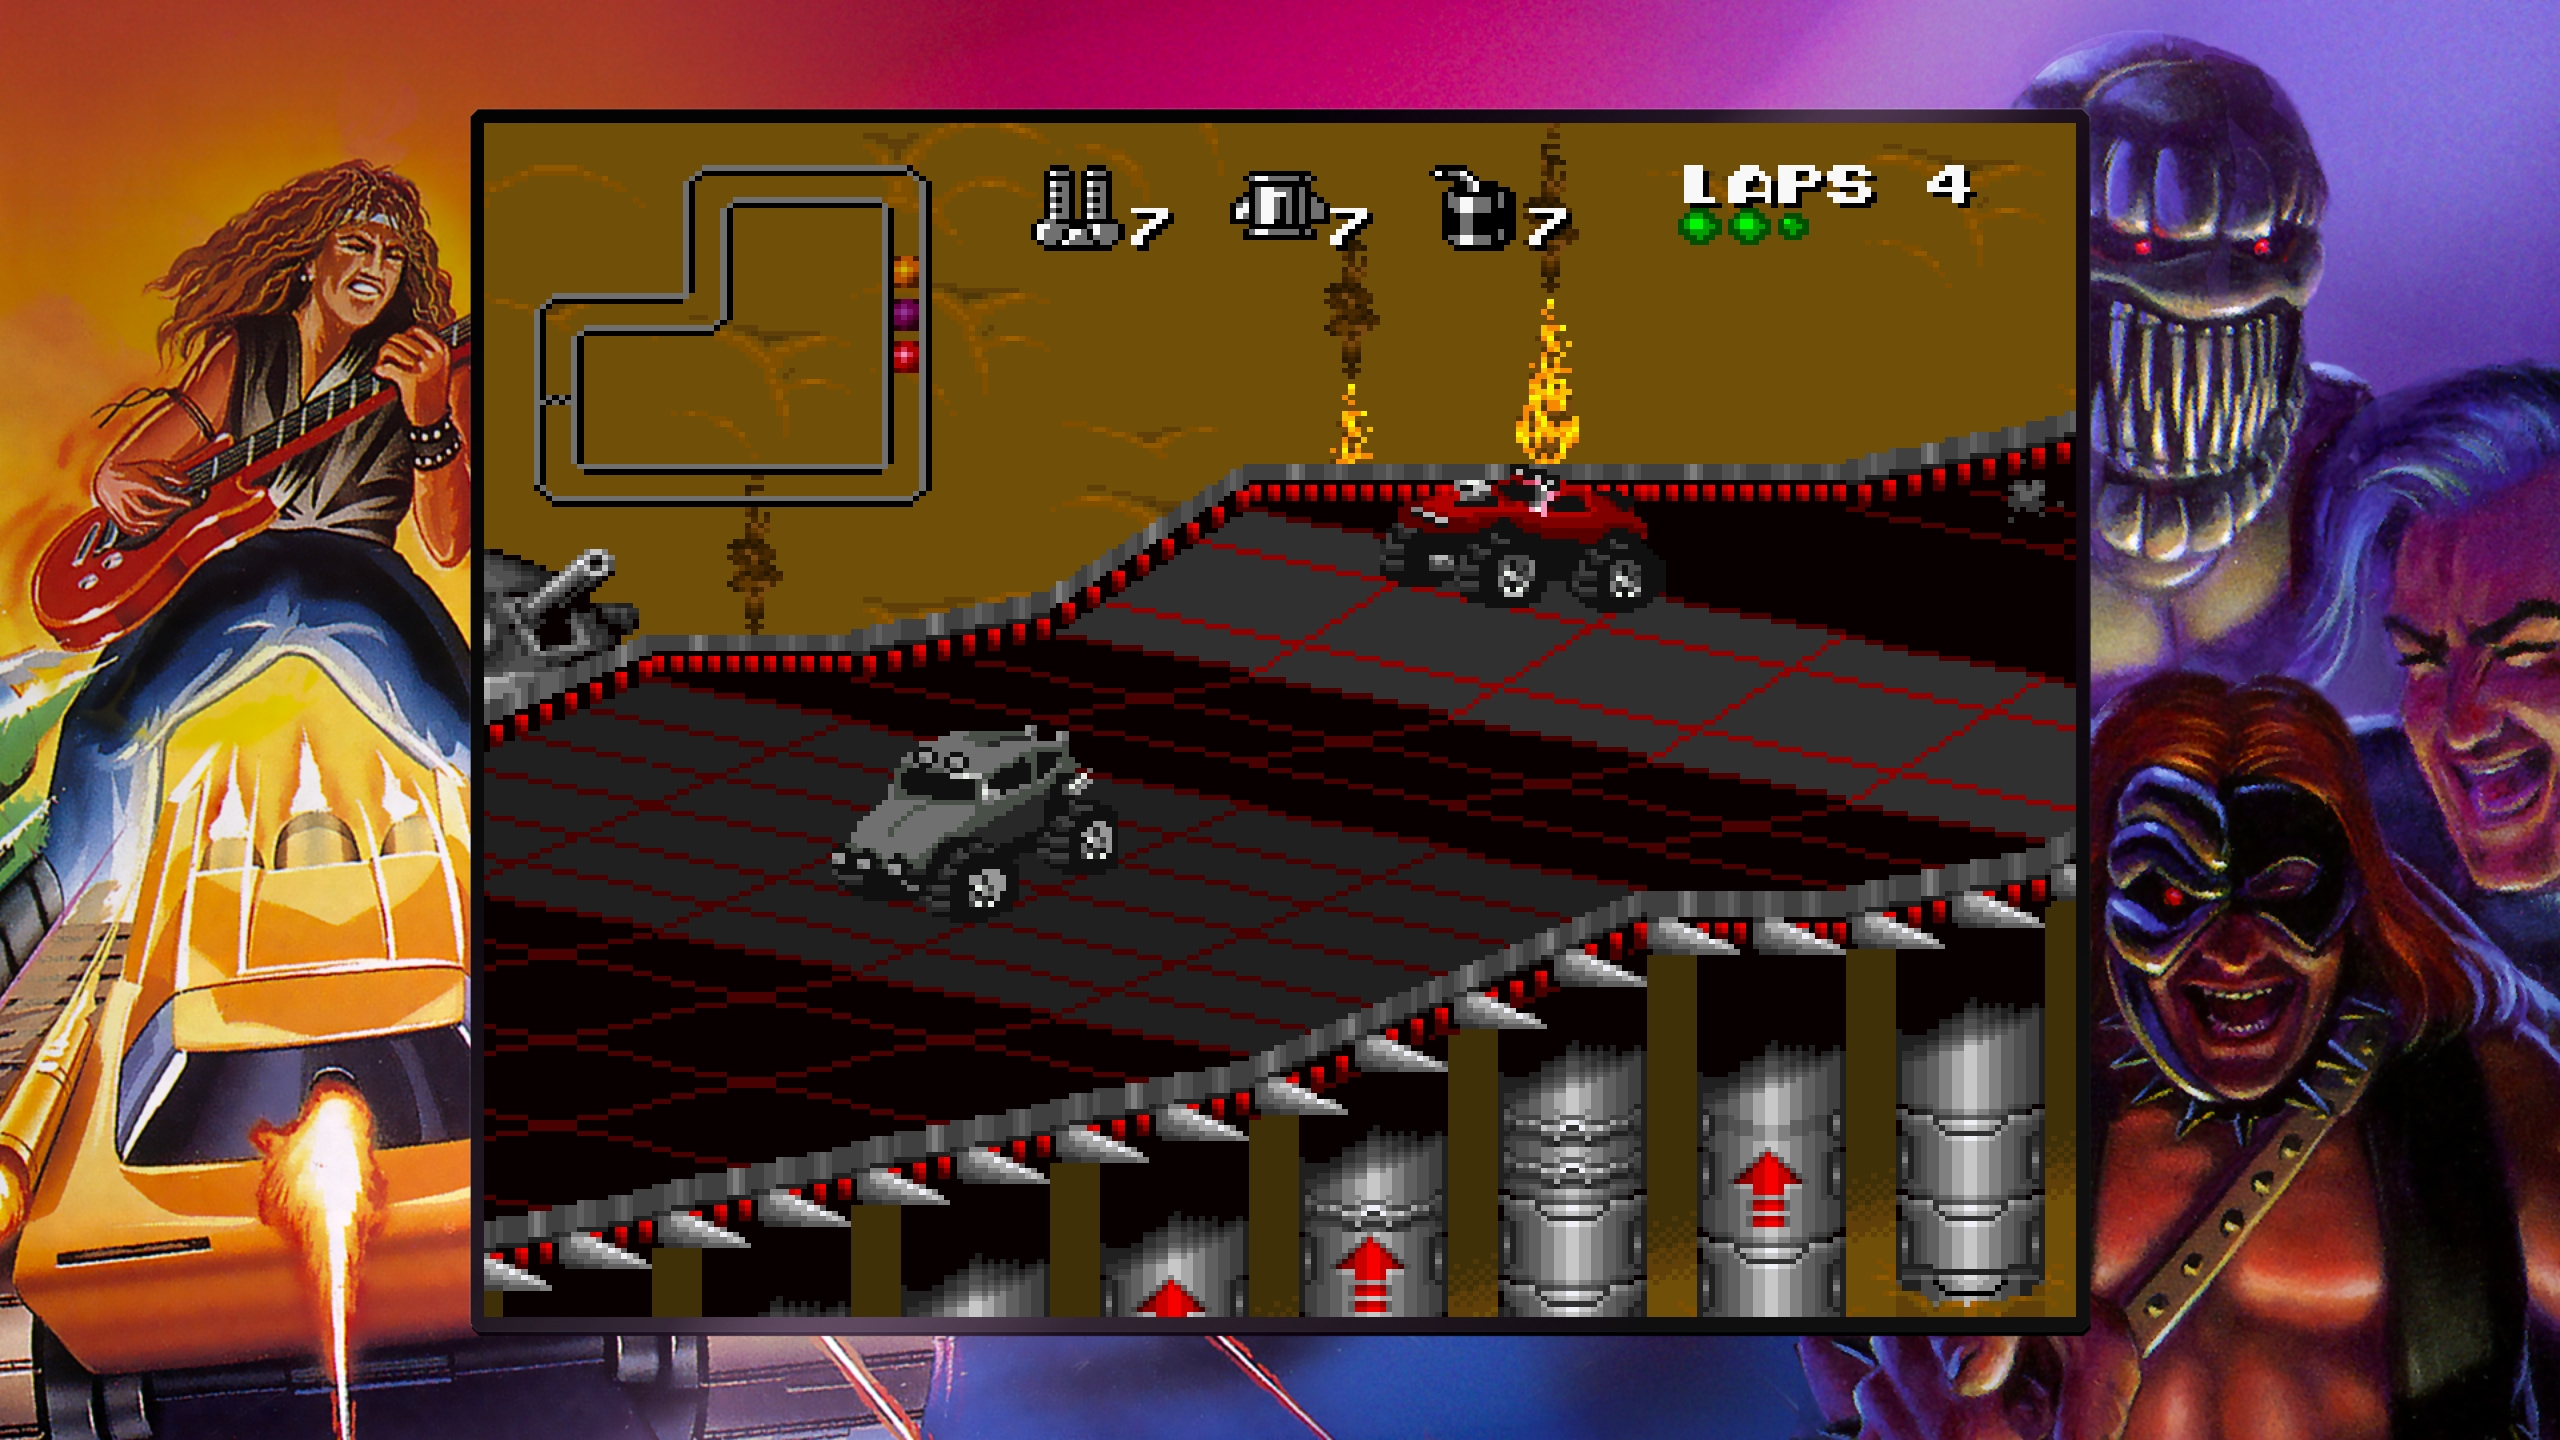
\includegraphics[width=0.8\textwidth]{figuras/Rock and Roll Racing.jpg}
    \caption{Rock \& Roll Racing. \cite{rockAndRollRacing}}
    \label{fig:rock-and-roll-racing}
\end{figure}

\section{Influência do gênero no mercado}

O gênero de corrida de Kart é muito popular e apreciado por muitos jogadores, de todas as idades e gêneros, e é um dos gêneros mais bem-sucedidos e lucrativos da indústria de jogos eletrônicos. Vários jogos de corrida de Kart já foram desenvolvidos e lançados para diferentes plataformas, como o SNES, PlayStation, Xbox, PC, entre outros, e muitos deles se tornaram grandes sucessos de crítica e público.

Além disso, o gênero de corrida de Kart é muito versátil e diversificado, o que permite a criação de jogos com diferentes estilos e mecânicas de jogo, que podem atrair diferentes categorias de jogadores e públicos. Por exemplo, \textit{Mario Kart} é conhecido por sua jogabilidade acessível e dinâmica, que combina elementos de corrida e combate, e por seus personagens carismáticos e coloridos, como Mario, Luigi, Peach, Bowser, Donkey Kong, Yoshi, entre outros.

\subsection{Sucesso financeiro}

A franquia \textit{Mario Kart} é uma das mais bem-sucedidas da Nintendo, com milhões de cópias vendidas em todo o mundo e vários jogos lançados para diferentes plataformas, como o SNES, Nintendo 64, GameCube, Wii, Wii U, Nintendo DS, Nintendo 3DS, Nintendo Switch, entre outros.

Hoje em dia, \textit{Mario Kart 8 Deluxe} é o jogo de corrida de Kart mais vendido de todos os tempos, com mais de 70.43 milhões de cópias vendidas em todo o mundo. A série \textit{Mario Kart} não só foi popular entre os jogos de corrida, já que além de ser o jogo mais vendido para o\textit{Nintendo Switch}, console da Nintendo, também é o sexto jogo mais vendido de todos os tempos, considerando todas as plataformas e gêneros (\cite{bestSellingGames}).

\begin{figure}[H]
    \centering
    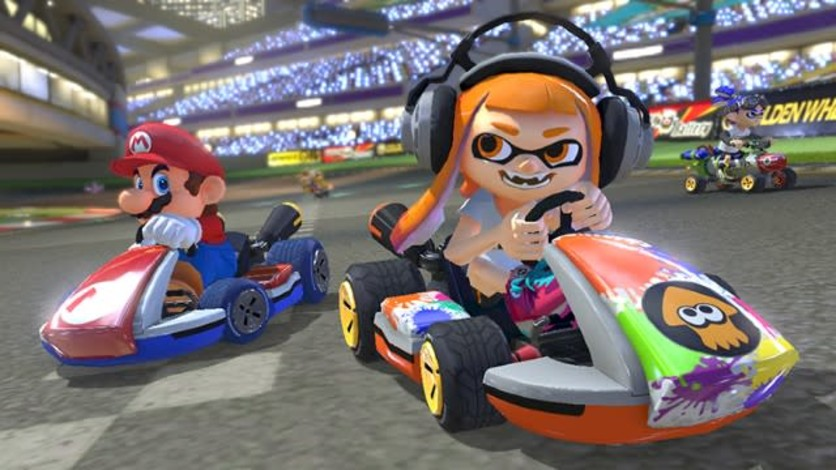
\includegraphics[width=0.8\textwidth]{figuras/Mario Kart 8.jpg}
    \caption{Mario Kart 8 Deluxe. \cite{marioKart8}}
    \label{fig:mario-kart-8-deluxe}
\end{figure}

\subsection{Impacto social}

O gênero inteiro de corrida de Kart é muito popular e apreciado por muitos jogadores, de todas as idades e gêneros, e é também tão importante que influenciou a cultura pop e a sociedade de várias maneiras.

Em uma pesquisa feita pela \textit{BonusFinder}, foi descoberto que \textit{Mario Kart} não é somente o jogo de corrida mais popular, mas também é o terceiro jogo mais estressante de todos os tempos. A pesquisa foi medindo o aumento da frequência cardíaca dos jogadores enquanto jogavam, e \textit{Mario Kart} aumentou a frequência cardíaca em 73.44\% (\cite{stressful:bonusFinder}). Isso mostra o quanto o jogo é popular e apreciado por muitos jogadores, de todas as idades e gêneros, e o quanto ele é importante para a cultura pop e a sociedade.